\chapter{Strategia prowadzenia prac}
\label{strategia_prac}

W tym rozdziale opisujemy metodologię prac nad poszczególnymi częściami projektu. Każda z nich była rozwijana
innym sposobem z powodu dużych rozbieżności specyfiki konkretnych problemów -- zupełnie inaczej pracuje się
nad semi-formalną specyfikacją języka programowania niż nad aplikacją użytkową, więc podjęliśmy decyzję o
rozdzieleniu tych części i poprowadzeniu ich jako osobne, mniejsze projekty wewnątrz pracy inżynierskiej.

\section{Specyfikacja języka \ViuAct}

Tworzenie specyfikacji języka odbywało się w modelu kaskadowo-prototypowym i
przeplatało się z implementacją prototypu kompilatora.

\subsection{Określenie wymagań}

Przed rozpoczęciem specyfikowania poszczególnych konstrukcji językowych należało
podjąć decyzję co w języku powinno się znaleźć, a co nie powinno zostać włączone
do specyfikacji. Pragmatyczne podejście pozwoliło ograniczyć do minimum liczbę
potrzebnych elementów języka -- zrezygnowano między innymi z umieszczenia pętli
w języku ponieważ można je zastąpić rekurencyjnymi wywołaniami w pozycji
ogonowej (\emph{recursive tail calls}).

\subsection{Specyfikacja konkretnej konstrukcji języka}

Każda konstrukcja językowa była najpierw projektowana, następnie dokumentowana i
omawiana (żeby wychwycić oczywiste błędy ,,grube'' na wczesnym etapie prac).
Potem proces specyfikacji zostawał zawieszony do momentu wytworzenia w
kompilatorze prototypu implementacji danej konstrukcji, lub odrzucenia jej jako
niewykonalnej w zakładanym czasie lub zakresie funkcjonalności. Na tym etapie
specyfikacja była ,,luźna'' i półformalna.

Wynik prac prototypowych (sukces bądź porażka) decydował o tym czy prace
specyfikacyjne były prowadzone dalej. Jeśli konstrukcja okazywała się możliwa
do zaimplementowania jej specyfikacja była formalizowana oraz przygotowywana
była jej dokumentacja (obejmująca m.in. przykłady użycia). Po tym etapie
specyfikacja była już w pełni formalna.

\section{Kompilator języka \ViuAct}

Prace nad kompilatorem języka \ViuAct\ były prowadzone w identyczny sposób jak
prace nad Viua~VM. Jest to połączenie strategii prototypowania i iteracji, które
spawdza się przy projekcie rozwijanym w stylu \emph{one-man show}, czyli tam
gdzie za cały projekt odpowiada jeden programista. Jest to częsta sytuacja w
przypadku projektów Free Software i na takim modelu wytwarzania był oparty
sposób wytworzenia kompilatora języka \ViuAct.

\subsection{Określenie wymagań}

Przed rozpoczęciem prac nad kompilatorem języka \ViuAct\ należało określić
wymagania jakie powinien spełnić. Z uwagi na krótki czas trwania projektu lista
wymagań musiała być krótka. Zaowocowało to rezygnacją z funkcjonalności
podnoszących \emph{quality of life} programisty korzystającego z
kompilatora, np. dokładnego raportowania błędów. Wymagania, które finalnie
zostały zaakceptowane są opisane w rozdziale \ref{viuact_zal_wymagania} na
stronie \pageref{viuact_zal_wymagania}.

\subsection{,,Swobodna'' strategia}

Strategia nie zakładała planowania znanych z Agile sprintów, przypisywania zadań
do konkretnych terminów, czy tworzenia złożonych \emph{workflow}. Jedynym planem
była lista zadań, które musiały być zrealizowane aby projekt został z sukcesem
ukończony i powiązanie ich w relacje \emph{zależy-od}, gdzie jeśli zadanie A
\emph{zależy-od} zadania B, to zadanie B musi być ukończone przed zadaniem A.
W wyniku takich powiązań powstało drzewo, które określało kolejność w jakiej
poszczególne zadania musiały być wykonywane.

Takie względnie ,,swobodne'' podejście do spraw planowania i formalnego
zarządzania projektem pozwoliło na drastyczne zminimalizowanie biurokratycznego
narzutu na projekt i umożliwiło przeznaczenie większej ilości czasu na prace
programistyczne bądź przygotowywanie dokumentacji.

\subsection{Narzędzia wspierające wybraną strategię}

Zadania w tej części projektu były śledzone za pomocą narzędzia
\texttt{issue}\footnote{Kod źródłowy dostępny jest pod adresem
\url{https://github.com/marekjm/issue}. Narzędzie to jest również krótko opisane
w dodatku \ref{issue_tracking_tool} na stronie \pageref{issue_tracking_tool}.},
które jest również wykorzystywane przez jednego z członków zespołu (Marka
Mareckiego) do śledzenia zadań w pracy zawodowej oraz jego projektach
Free~Software i bezpośrednio wspiera opisane powyżej ,,swobodne'' podejście do
zarządzania zadaniami w projekcie.

Prace implementacyjne przeplatały się z pracami nad specyfikacją w celu
weryfikowania na bieżąco co jest możliwe do wykonania w zamierzonym czasie w
całości, co tylko w części, a co nie jest możliwe do wykonania przy zakładanych
zasobach czasowo-ludzkich.

\subsection{Testowanie}

Prace nad kompilatorem języka \ViuAct\ były ,,pilnowane'' przez zestaw testów, w
którym każdy test był prostym, ale kompletnym programem testowym.

Każdy test sprawdza czy dany program poprawnie się kompiluje i czy po wykonaniu
daje oczekiwane wyniki. Ta strategia -- brak testów poszczególnych elementów
kompilatora, a jedynie weryfikacja, że całość działa poprawnie -- została
zaadaptowana z projektu Viua~VM, gdzie jest z powodzeniem wykorzystywana.
Zapewnia ona maksimum zysków przy minimum narzutu i kosztów czasowych:

\begin{enumerate}
    \item wiemy, że kompilator jako całość działa ponieważ każdy z programów
        testowych
        \begin{enumerate*}[label=(\arabic*)]
            \item jest możliwy do skompilowania
            \item daje oczekiwane wyniki
        \end{enumerate*}
    \item traktujemy kompilator jako ,,czarną skrzynkę'' i nie testujemy wnętrza
        kompilatora, a jedynie weryfikujemy czy poprawnie przetwarza kod
        źródłowy na kod wynikowy co pozwala na dowolne manipulowanie
        implementacją bez zmiany testów
\end{enumerate}

Takie podejście wymaga częstego uruchamiania testów w celu weryfikacji czy
zmiany, które wprowadzamy nie powodują porażki wykonania zestawu testowego --
łatwiej jest znaleźć błąd w czterech liniach zmian niż w czternastu czy
czterdziestu -- ponieważ taki zestaw testów nie jest pomocny w szukaniu błędów w
implementacji. Świadomie podjęliśmy decyzję o przyznaniu większej wagi temu żeby
sprawdzić czy w zakładanych przypadkach kompilator zachowuje się poprawnie niż
na temu żeby testy pomagały w wyszukiwaniu błędów ponieważ, z uwagi na bardzo
ograniczony czas na jego wytworzenie, ważniejsze było osiągnięcie przez
kompilator ,,kompletności'' niż jego odporność na błędy.

\section{Program ViuaChat}

\subsection{mini-Scrum}
Dla czatu ViuaChat, Krzysztof Franek, odpowiedzialny za tę część projektu, wybrał strategię mini-Scrum. Jest to
wariant techniki Scrum, korzystający z tych podobnych wydarzeń (Sprint, Planowanie Sprintu, Przegląd Sprintu,
Retrospektywa Sprintu), tych samych artefaktów (Backlog Produktu, Backlog Sprintu, Przyrost) i niektórych ról
(Właściciel Produktu, Zespół Deweloperski).

Podstawową zaletą tej metodyki działania był podział zadań na mniejsze fragmenty, a także możliwość łatwego
planowania i nadzorowania tempa prac poprzez obserwowanie wykresu wypalania produktu. Umówiono się, że rolę
właściciela produktu (ang. \textit{product owner}) będzie pełnił p. Marecki, zaś w rolę zespołu deweloperskiego
wcieli się p. Franek. Z powodu mało licznego zespołu, w metodologi mini-Scrum dokonano pewnych uproszczeń w
stosunku do oryginalnego modelu Scruma, zaproponowanego w oficjalnym podręczniku (\cite{Scrum}). Zrezygnowano
z codziennych scrumów (ang. \textit{daily scrums}), z uwagi na nieregularny charakter prac (uczestnicy projektu
studiują w trybie zaocznym i realizują zadania w czasie wolnym od pracy), a także z odrębnej roli \textit{scrum
mastera}.

\subsubsection{Kanban}
Dodatkowo, jako technikę prowadzenia Sprintów mini-Scruma wybrano Kanban, w ramach którego każda z historyjek
w Sprincie była umieszczana w postaci ,,karteczki'' na wirtualnej tablicy i przemieszczana pomiędzy jej kolumnami,
wraz z ich kolejnymi etapami realizacji. Na tablicy przewidziano następujące kolumny: ,,Do zrobienia'', ,,W
realizacji'', ,,W testowaniu'', ,,Zrealizowano''. Ponadto, każda karteczka ma przypisaną etykietę z priorytetem.

Początkowo, dla każdego sprintu  utworzona osobną tablicę. Karteczki reprezentujące historyjki, których nie udało się
zrealizować w sprincie, miały być kopiowane do tablic kolejnych sprintów. Ostatecznie poprzestano na uproszczonym toku postępowania, współdzielącym
jedną tablicę dla wszystkich sprintów -- karteczki
ze zrealizowanymi i przetestowanymi zadaniami poddawano archiwizacji, zaś
niezrealizowane wyróżniano dodatkową, ostrzegawczą etykietą.

Oprogramowanie zaproponowane do utrzymywania mini-Scruma dla ViuaChat to Trello, umożliwiające łatwe
zaimplementowanie techniki Kanban, rejestrowanie czasu pracy oraz integrację z najpopularniejszymi
dostarczycielami repozytoriów Git.

\subsection{Testowanie}

Proces testowania systemu ViuaChat został rozbity na dwa, odrębne poziomy,
realizowane w sposób równoległy.

Pierwszy z poziomów dotyczył testów jednostkowych backendu ViuaChat, tj. części systemu ViuaChat, która działa po stronie serwera. Aby zweryfikować działanie poszczególnych
komend oraz prawidłowość zwracanych rezultatów, przygotowywane były specjalnie
spreparowane pliki HTML. Ich esencją były osadzone skrypty w języku JavaScript,
które samoczynnie próbowały łączyć się z serwerem czatu, a w razie sukcesu
wysyłały serię zdefiniowanych komend. Przebieg komunikacji w był prezentowany
w przeglądarce internetowej.

\begin{figure}[!htp]
	\centering
	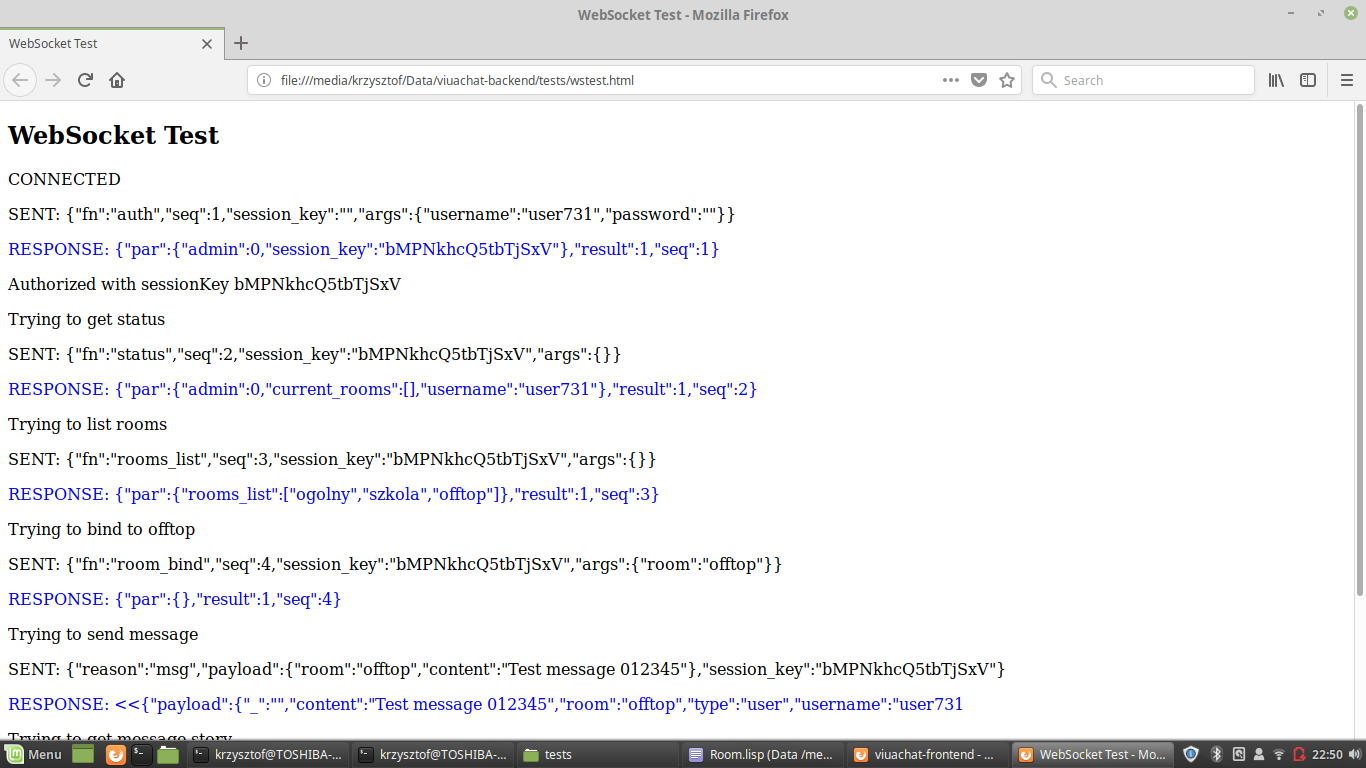
\includegraphics[width=\textwidth]{strategia/fig/testyws}
	\caption{Skrypt służący do zautomatyzowanych testów backendu ViuaChat}
	\label{testy-ws}
\end{figure}

Drugi z poziomów obejmował typowe testy integracyjne. Proces testowania
niejako ,,wbudowano'' w metodologię mini-Scrum. Wynika to z faktu, iż każda
z historyjek oraz każde z zadań posiada jasno określoną definicję ukończenia
(ang. \textit{Definition of Done}, \textit{DoD}). Nie było zatem możliwe jego
ukończenie bez spełnienia z góry określonych warunków.
